%%% Local Variables:
%%% mode: latex
%%% TeX-master: "report_main"
%%% End:

\section{Part 1 - Mathematical modeling}
\subsection{Problem 1}
\label{subsec:problem 1}
%
We use the helicopter model shown in \cref{fig:helicopter_model_forces} and
\cref{fig:helicopter_model_masses} as our starting point for deriving
the equations of motion.
%
\begin{figure}[hbp]
  \caption{the helicopter model figure 7 from the assignment depicting
    forces and joint axes \cite[p.12]{assignment}.}
  \label{fig:helicopter_model_forces}
  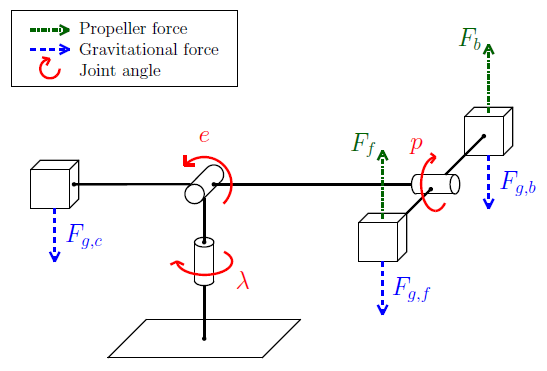
\includegraphics[width=\textwidth]{images/helicopter_model_forces}
\end{figure}
%
\begin{figure}[H]
  \caption{the helicopter model figure 8 from the assignment depicting
    masses and distances between the joint axes and the point masses
    \cite[p.13]{assignment}.}
  \label{fig:helicopter_model_masses}
  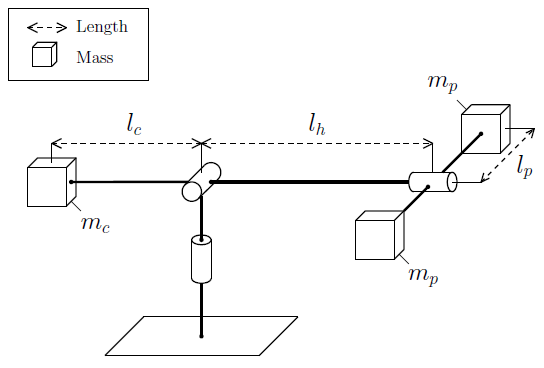
\includegraphics[width=\textwidth]{images/helicopter_model_masses}
\end{figure}
%
Only forces perpendicular to a moment arm, with the moment arm again
perpendicular to the axis of rotation in question produces moment, or
torque. The equation of motion for the pitch is found through the
momentum around the pitch axis in the clockwise direction as shown in
\cref{fig:helicopter_model_forces}. It becomes:
%
\begin{align*}
  J_p\ddot{p} &= l_p(F_{g,b} - F_b - F_{g,f} + F_f) \\
              &= l_p(m_pg - mp_g + K_fV_f - V_b) \\
              &= l_pK_f(V_f-V_b)
\end{align*}
%
Where the lengths including $l_p$ is shown in
\cref{fig:helicopter_model_masses}. Since $V_d = V_f-V_b$, we can
write this as:
%
\begin{equation}
  \label{eq:pitch EoM}
  J_p\ddot{p} = l_pK_fVd
\end{equation}
Therefore $L_1 = l_pK_f$.

The equation of motion for the elevation angle is found similarly
through the momentum in the counter-clockwise direction around the
elevation axis, again as shown in
\cref{fig:helicopter_model_forces}.
%
\begin{equation*}
  J_e\ddot{e} = arm_cF_{g,c} - arm_h(F_{g,f}+F_{g,b}) + l_h(F_{f,p} + F_{b,p})
\end{equation*}
%
where $arm_c$ is the moment arm between the counterweight point mass
and the elevation axis, and $arm_h$ is the moment arm between any of
the two motor point masses and the elevation axis. $F_{f,p} =
F_{f,perpendicular}$ is the perpendicular component of $F_f$, and
$F_{b,p} = F_{b,perpendicular}$ is the perpendicular component of
$F_b$. As shown in \cref{fig:elevation_model}, $arm_c = l_ccos(e)$,
and $arm_h = l_hcos(e)$, and the moment arm for the motor forces is indeed $l_h$.
%
\begin{figure}[H]
  \caption{moment arms around the elevation axis, with relevant
    forces. Also, the positive direction of momentum is displayed as
    counter-clockwise around the e-axis.}
  \label{fig:elevation_model}
  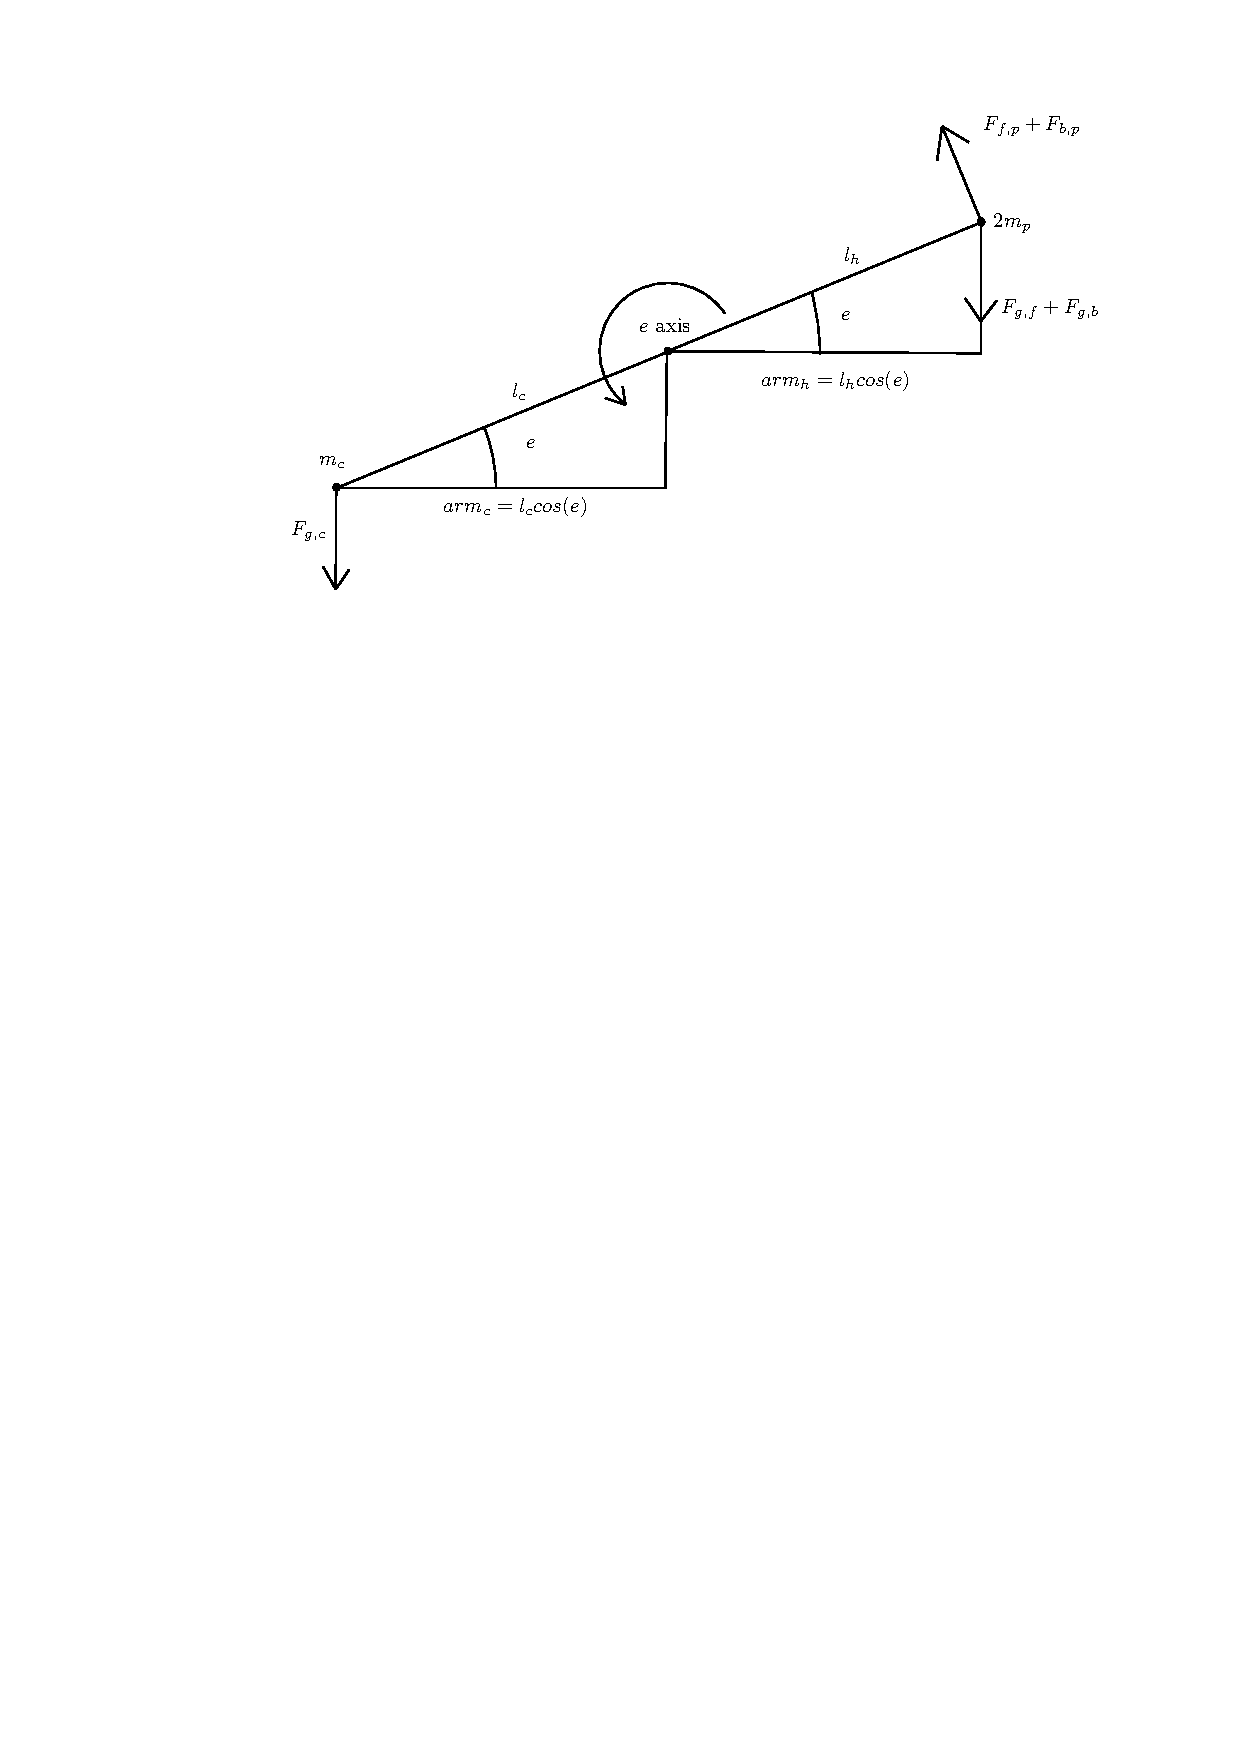
\includegraphics[width=1\textwidth]{images/elevation_model}
\end{figure}
\begin{figure}[H]
  \caption{gravitational and motor forces on the helicopter head, as
    well as the decomposition of the motor forces into vertical and
    horizontal components.}
  \label{fig:pitch_model}
  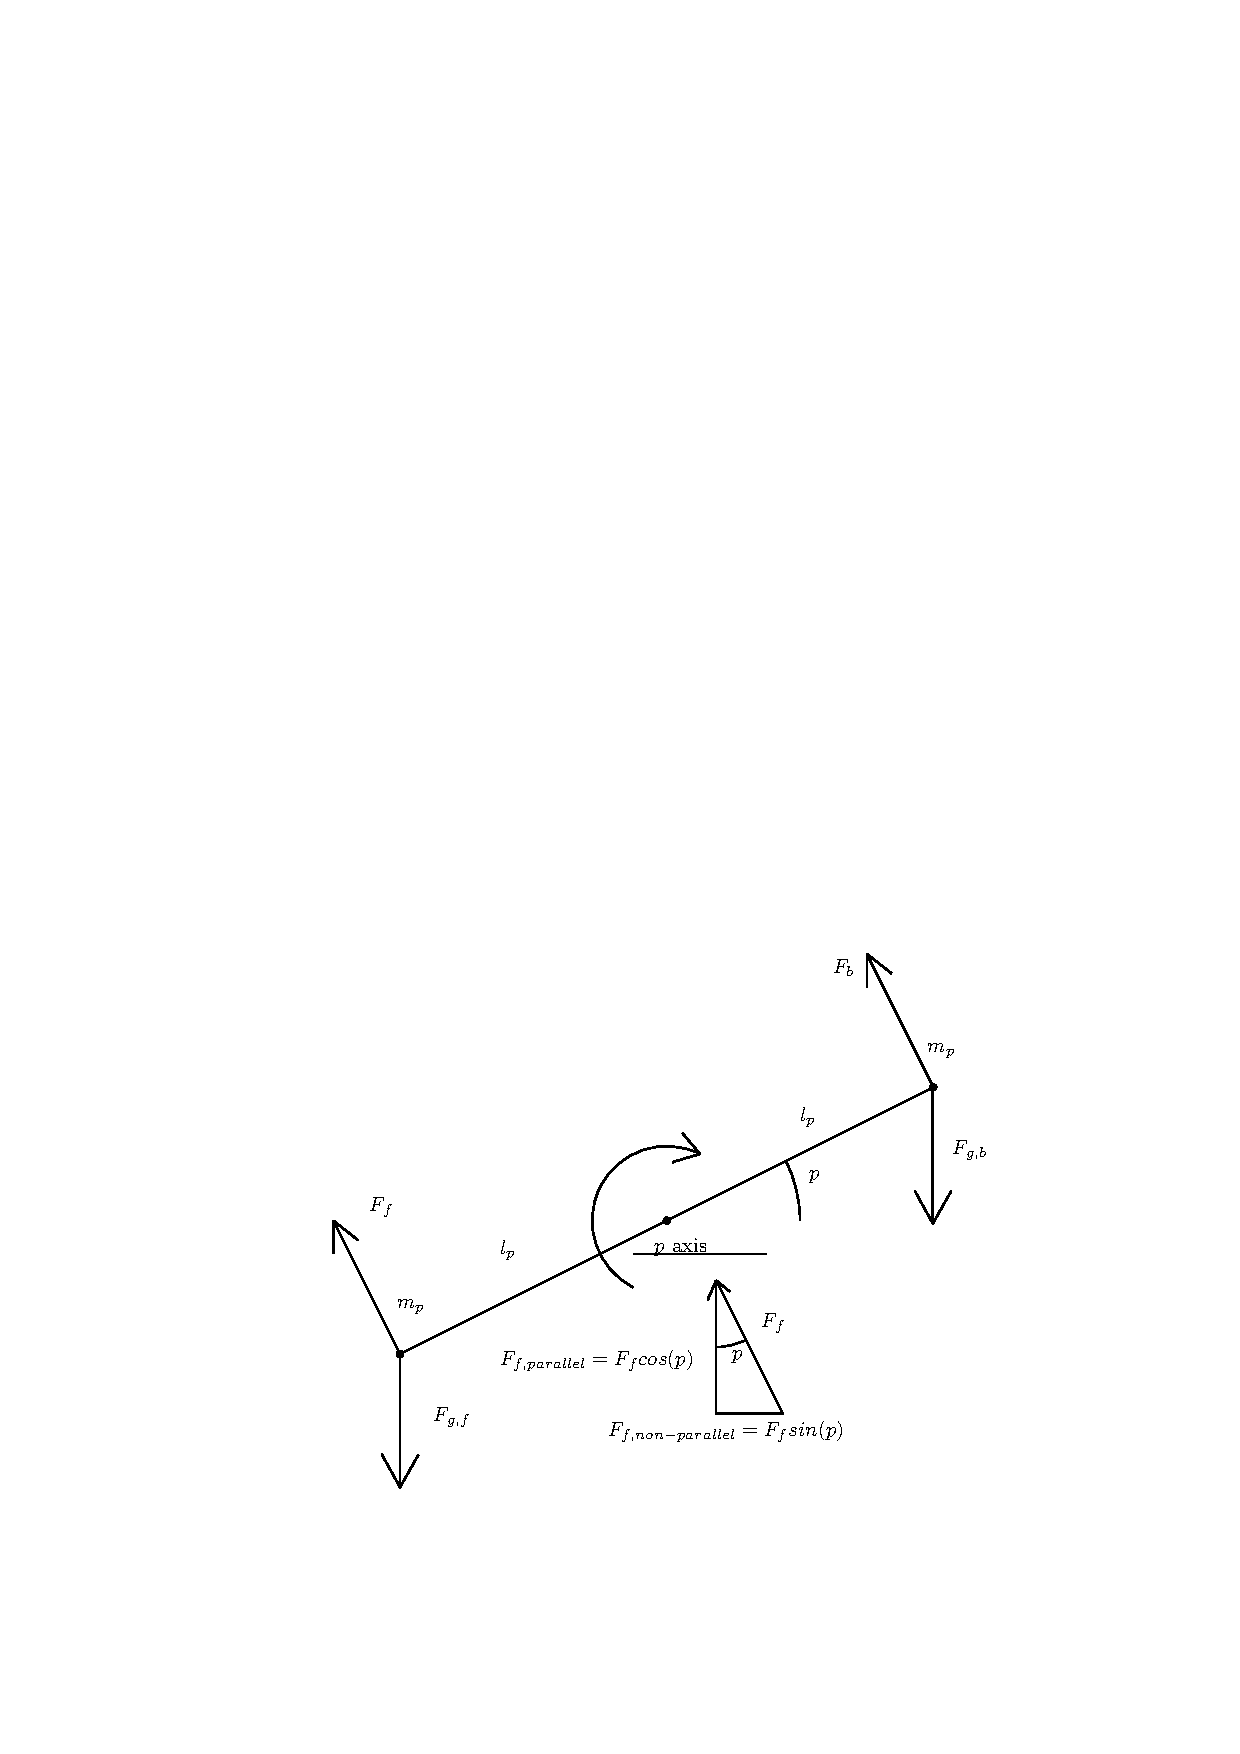
\includegraphics[width=1\textwidth]{images/pitch_model}
\end{figure}
%
As shown in \cref{fig:pitch_model}, the perpendicular components of the
motor forces $F_{f,p}$ and $F_{b,p}$ are $F_fcos(p)$ and $F_bcos(p)$
respectively.
%
\begin{align*}
  J_e\ddot{e} &= arm_cF_{g,c} - arm_h(F_{g,f}+F_{g,b}) + l_hcos(p)(F_f + F_b)) \\
              &= arm_cm_cg - arm_h(m_pg + m_pg) + l_hK_fcos(p)(V_f + V_b))
\end{align*}
%
We substitute in $V_s = V_f + V_b$ and the two moment arms:
%
\begin{align*}
  J_e\ddot{e} = l_ccos(e)m_cg - l_hcos(e)2m_pg + l_hK_fcos(p)V_s)
\end{align*}
The eqation of motion for the elevation angle then has the final form:
\begin{equation}
  \label{eq:elevation EoM}
  J_e\ddot{e} = g(l_cm_c - 2l_hm_p)cos(e) + l_hK_fV_scos(p)
\end{equation}
%
We see that $L_2 = g(l_cm_c-2l_hm_p)$, and $L_3 = l_hK_f$.
\\ \\
Finally, the equation of motion for the travel angle is found through
the momentum around the travel axis in the  clockwise direction, as
shown in \cref{fig:helicopter_model_forces}. As seen in
\cref{fig:pitch_model}, the only forces with a moment arm
perpendicular to the travel axis are the components of the motor
forces in the horizontal direction, $F_{f,h} = F_fsin(p)$ and $F_{b,h}
= F_bsin(p)$, has \cref{fig:elevation_model} have the moment arm of
length $arm_h = l_hcos(e)$:
%
\begin{align*}
  J_\lambda\ddot{\lambda} &= arm_h(F_{f,h} + F_{b,h}) \\
                         &= l_hcos(e)(K_fsin(p)(V_f + V_b))
\end{align*}
%
Again substituting $V_s = V_f + V_b$, and we get the final equation of
motion for the travel angle:
%
\begin{equation}
  \label{eq:travel EoM}
  J_\lambda\ddot{\lambda} = l_hK_fV_scos(e)sin(p)
\end{equation}
%
We see that $L_4 = l_hK_f$.

\Crefrange{eq:pitch EoM}{eq:travel EoM} respectively correspond to equations
(2a) to (2c) from the assignment \cite[p.13]{assignment}.
%
\subsection{Problem 2}
To linearize the system about the point with all state variables equal
to zero ($(p, e, \lambda)^T = (\dot{p},\dot{e},\dot{\lambda})^T $ = (0, 0, 0))
the inputs in the equations of motion ($V^{*}_{s} \text{ and }
V^{*}_{d}$) must be set to values that make this an equilibrium point.

At the linearization point, the equation of motion for pitch,
\cref{eq:pitch EoM}, reduces to $0 = L_{1} *
V^{*}_{d}$ therefore:
%
\begin{equation}
  \label{eq:V^*_d value}
  V^{*}_{d} = 0
\end{equation}
At the linearization point, the equation of motion for elevation,
\cref{eq:elevation EoM}, reduces to $0 = L_{2} +
L_{3}*V^{*}_{s}$ therefore:
%
\begin{equation}
  \label{eq:V^*_s value}
  V^{*}_{s} = -L_{2} / L_{3}
\end{equation}
%
While the equation of motion for travel, \cref{eq:travel EoM}, at the
linearization point simply reduces to 0 = 0.
The following transformation is performed to simplify the analysis
\cite[p.14]{assignment}:
%
\begin{equation}
  \label{eq:transformation}
  \begin{bmatrix}
    \tilde{p} \\
    \tilde{e} \\
    \tilde{\lambda}
  \end{bmatrix}
  =
  \begin{bmatrix}
    p \\
    e \\
    \lambda
  \end{bmatrix}
  -
  \begin{bmatrix}
    p^{*} \\
    e^{*} \\
    \lambda^{*}
  \end{bmatrix}
  and
  \begin{bmatrix}
    \tilde{V}_{s} \\
    \tilde{V}_{d}
  \end{bmatrix}
  =
  \begin{bmatrix}
    V_{s} \\
    V_{d}
  \end{bmatrix}
  -
  \begin{bmatrix}
    V^{*}_{s} \\
    V^{*}_{d}
  \end{bmatrix}
\end{equation}
%
The equations of motion in the transformed system are therefore:
%
\begin{subequations}
  \begin{align}
    J_p\ddot{\tilde{p}} &= L_1\tilde{V_d}
    \label{eq:transformed pitch EoM}\\
    J_e\ddot{\tilde{e}} &=
    L_2cos(\tilde{e}) + L_3(\tilde{V_s}+L_2/L_3)cos(\tilde{p})
    \label{eq:transformed elevation EoM}\\
    J_{\lambda}\ddot{\tilde{\lambda}} &=
    L_4(\tilde{V_s}+L_2/L_3)cos(\tilde{e})sin(\tilde{p})
    \label{eq:transformed travel EoM}
  \end{align}
\end{subequations}
%
By choosing the state to be x = ($\tilde{p}$, $\tilde{e}$,
$\tilde{\lambda}$, \textit{$\dot{p}$, $\dot{e}$,$\dot{\lambda}$}) the
nonlinear state equations become:
%
\begin{subequations}
  \label{eq:full state equations}
  \begin{align}
    \dot{x}_1 &= x_4 \\
    \dot{x}_2 &= x_5 \\
    \dot{x}_3 &= x_6 \\
    \dot{x}_4 &= (L_1/J_p) V_d \\
    \dot{x}_5 &= (L_2/J_e)cos(x_2) + (L_3/J_e)(V_s + L_2 / L_3)cos(x_1) \\
    \dot{x}_6 &= (L_4 / J_\lambda) (V_s + L_2 / L_3)cos(x_2)sin(x_1)
  \end{align}
\end{subequations}
If the above system is expressed as $\dot{x} = h(x, u)$, where x is
the state and u is the input, the system is linearized by finding the
Jacobians of h with respect to the state and the input and then
inserting the equilibrium values.
%
\begin{equation}
  \label{eq:Linearized Jacobians}
  \frac{\partial h}{\partial x} = A =
  \begin{bmatrix}
    0 & 0 & 0 & 1 & 0 & 0 \\
    0 & 0 & 0 & 0 & 1 & 0 \\
    0 & 0 & 0 & 0 & 0 & 1 \\
    0 & 0 & 0 & 0 & 0 & 0 \\
    0 & 0 & 0 & 0 & 0 & 0 \\
    \frac{L_4L_2}{J_\lambda L_3} & 0 & 0 & 0 & 0 & 0
  \end{bmatrix}
  \qquad
  \frac{\partial h}{\partial u} = B =
  \begin{bmatrix}
    0 & 0 \\
    0 & 0 \\
    0 & 0 \\
    0 & L_1/J_p \\
    L_3/J_e & 0 \\
    0 & 0
  \end{bmatrix}
\end{equation}
where $L_1, L_2, L_3$ and $L_4$ were calculated in
\cref{subsec:problem 1} and $J_p, J_e$ and $J_\lambda$ were given in
the assignment description \cite[p.14]{assignment}.
%
The linearized equations of motion can therefore be written in the
following form:
%
\begin{subequations}
  \label{eq:linearized EoM}
  \begin{align}
    \ddot{\tilde{p}} &=
    K_1\tilde{V}_d \qquad K_1 = \frac{L_1}{J_p}
    \label{eq:linearized pitch EoM}\\
    \ddot{\tilde{e}} &=
    K_2\tilde{V}_s \qquad K_2 = \frac{L_3}{J_e}
    \label{eq:linearized elevation EoM}\\
    \ddot{\tilde{\lambda}} &=
    K_3\tilde{p} \qquad K_3 = \frac{L_4L_2}{J_\lambda L_3}
    \label{eq:linearized travel EoM}
  \end{align}
\end{subequations}

\subsection{Problem 3}
\todo[inline]{Check if we added gain to the output of joystick}
The helicopter is difficult to control using only feed-forward. The
physical behaviour of the helicopter differs from the (2a) - (2c)
\cite[p.13]{assignment} model because it does not take into
consideration drag, ground effects, etc.

In \cref{eq:linearized EoM} the model is linearized around a point with
all angles equal to zero, where elevation is defined as zero when the
elevation arm is parallel to the table, pitch is defined as zero when
the pitch arm is parallel to the table and travel angle is defined as
zero at the initial travel angle. Since the physical system is not
linear, the linear assumption breaks down when the system is too far
from this point.

\subsection{Problem 4}
Elevation is the only variable that needs to be changed, since travel
and pitch are zeroed correctly upon initialization. To correct for the
offset of the arm at startup, subtract 30 degrees from the elevation
to get the correct point of zero elevation.

The value of $V^*_s$ in order to stabilize the helicopter at the
equilibrium point, was measured to be 7.5 V.

The motor force constant, $K_f$, which relates $F_f$ and $V_f$ is
calculated to be $-(L_2/l_h)*V^*_s$, and has the value 0.1332.


%%% Local Variables:
%%% mode: latex
%%% TeX-master: "report_main"
%%% End:
